\chapter{Mechanics}
\section{Relating velocities}
Always remember to draw vector triangles to try to relate velocities of objects.
\begin{mybox}{gray}{Example from \textbf{Morin 8.16}}
    Basically part of the question requires us to relate the relative velocity between the 3 identical cylinders (2 below, 1 on top)
    \begin{flushleft}
        In this question, we don't really have to care about whether the circles are rolling, or sliding. As long as the surfaces are always in contact with each other, rolling and sliding will be the same.
    \end{flushleft}
    \begin{flushleft}
        The top cylinder (A) is moving vertically downwards. Its \textbf{instantaneous} resultant velocity can be seen as a vector summation of its motion of sliding down one of the bottom cylinder, B (slide down along the tangent of the contact point) and moving together with the bottom cylinder to the right.
    \end{flushleft}
    \begin{equation}
        \vec{v}_B=\vec{v}_{B,A}+\vec{v}_A
    \end{equation}
\end{mybox}

\begin{figure}[h]
    \centering
    \tikzset{every picture/.style={line width=0.75pt}} %set default line width to 0.75pt        
    \begin{tikzpicture}[x=0.75pt,y=0.75pt,yscale=-0.7,xscale=0.7]
        %uncomment if require: \path (0,264); %set diagram left start at 0, and has height of 264

        %Shape: Ellipse [id:dp6454937638049347] 
        \draw  [fill={rgb, 255:red, 225; green, 225; blue, 225 }  ,fill opacity=1 ] (137.17,88.93) .. controls (137.17,58.04) and (162.21,33) .. (193.1,33) .. controls (224,33) and (249.04,58.04) .. (249.04,88.93) .. controls (249.04,119.82) and (224,144.87) .. (193.1,144.87) .. controls (162.21,144.87) and (137.17,119.82) .. (137.17,88.93) -- cycle ;
        %Shape: Ellipse [id:dp09659041693487258] 
        \draw  [fill={rgb, 255:red, 225; green, 225; blue, 225 }  ,fill opacity=1 ] (79,185.14) .. controls (79,154.25) and (104.04,129.21) .. (134.93,129.21) .. controls (165.82,129.21) and (190.87,154.25) .. (190.87,185.14) .. controls (190.87,216.03) and (165.82,241.07) .. (134.93,241.07) .. controls (104.04,241.07) and (79,216.03) .. (79,185.14) -- cycle ;
        %Shape: Circle [id:dp7523877018092493] 
        \draw  [fill={rgb, 255:red, 225; green, 225; blue, 225 }  ,fill opacity=1 ] (193.1,185.14) .. controls (193.1,154.25) and (218.15,129.21) .. (249.04,129.21) .. controls (279.93,129.21) and (304.97,154.25) .. (304.97,185.14) .. controls (304.97,216.03) and (279.93,241.07) .. (249.04,241.07) .. controls (218.15,241.07) and (193.1,216.03) .. (193.1,185.14) -- cycle ;
        %Straight Lines [id:da7934319805293468] 
        \draw    (80.79,241.52) -- (304.52,241.52) ;
        %Shape: Ellipse [id:dp9436597516501397] 
        \draw  [fill={rgb, 255:red, 225; green, 225; blue, 225 }  ,fill opacity=1 ] (403.41,88.93) .. controls (403.41,58.04) and (428.46,33) .. (459.35,33) .. controls (490.24,33) and (515.28,58.04) .. (515.28,88.93) .. controls (515.28,119.82) and (490.24,144.87) .. (459.35,144.87) .. controls (428.46,144.87) and (403.41,119.82) .. (403.41,88.93) -- cycle ;
        %Shape: Ellipse [id:dp5128552258927073] 
        \draw  [fill={rgb, 255:red, 225; green, 225; blue, 225 }  ,fill opacity=1 ] (345.24,185.14) .. controls (345.24,154.25) and (370.29,129.21) .. (401.18,129.21) .. controls (432.07,129.21) and (457.11,154.25) .. (457.11,185.14) .. controls (457.11,216.03) and (432.07,241.07) .. (401.18,241.07) .. controls (370.29,241.07) and (345.24,216.03) .. (345.24,185.14) -- cycle ;
        %Shape: Ellipse [id:dp21704569705186105] 
        \draw  [fill={rgb, 255:red, 225; green, 225; blue, 225 }  ,fill opacity=1 ] (459.35,185.14) .. controls (459.35,154.25) and (484.39,129.21) .. (515.28,129.21) .. controls (546.17,129.21) and (571.21,154.25) .. (571.21,185.14) .. controls (571.21,216.03) and (546.17,241.07) .. (515.28,241.07) .. controls (484.39,241.07) and (459.35,216.03) .. (459.35,185.14) -- cycle ;
        %Straight Lines [id:da9042183550203948] 
        \draw    (347.03,241.52) -- (570.77,241.52) ;
        %Straight Lines [id:da8134842484634719] 
        \draw [color={rgb, 255:red, 245; green, 166; blue, 35 }  ,draw opacity=1 ][line width=2.25]    (575.24,81.67) -- (399.61,192.42) ;
        %Straight Lines [id:da47693545074586075] 
        \draw [color={rgb, 255:red, 208; green, 2; blue, 27 }  ,draw opacity=1 ][line width=2.25]    (193.1,88.93) -- (134.93,185.14) ;
        %Straight Lines [id:da8341487281668398] 
        \draw [color={rgb, 255:red, 208; green, 2; blue, 27 }  ,draw opacity=1 ][line width=2.25]    (249.04,185.14) -- (134.93,185.14) ;
        %Straight Lines [id:da8027791787204905] 
        \draw [color={rgb, 255:red, 208; green, 2; blue, 27 }  ,draw opacity=1 ][line width=2.25]    (249.04,185.14) -- (193.1,88.93) ;
        %Straight Lines [id:da27035493326436333] 
        \draw [color={rgb, 255:red, 208; green, 2; blue, 27 }  ,draw opacity=1 ][line width=2.25]    (513.94,186.48) -- (459.35,88.93) ;
        %Straight Lines [id:da5901311794622432] 
        \draw [color={rgb, 255:red, 208; green, 2; blue, 27 }  ,draw opacity=1 ][line width=2.25]    (579.72,137.48) -- (435.41,137.48) ;

        % Text Node
        \draw (200,158) node [anchor=north west][inner sep=0.75pt]    {$60^0$};
        % Text Node
        \draw (523,110) node [anchor=north west][inner sep=0.75pt]    {$30^0$};


    \end{tikzpicture}

\end{figure}

\section{Friction}
\subsection{Friction on inclined slope}
If a body is on the verge of slipping (or already slipping), then the sum of the friction force and the reaction force is angled by $\arctan{\mu}$ from the surface normal. This is actually quite useful in certain questions. \textcolor{blue}{\textit{Sometimes, we don't even have to resolve forces by projecting their components onto axes. We can instead add them up vectorially by drawing vector diagram (head to tail).}} This can be shown in the example below from \textit{Jaan Kalda's Mechanics handout}.

\begin{mybox}{gray}{Mechanics \textbf{pr 5.}}
    \begin{wrapfigure}{l}{0.6\textwidth}
        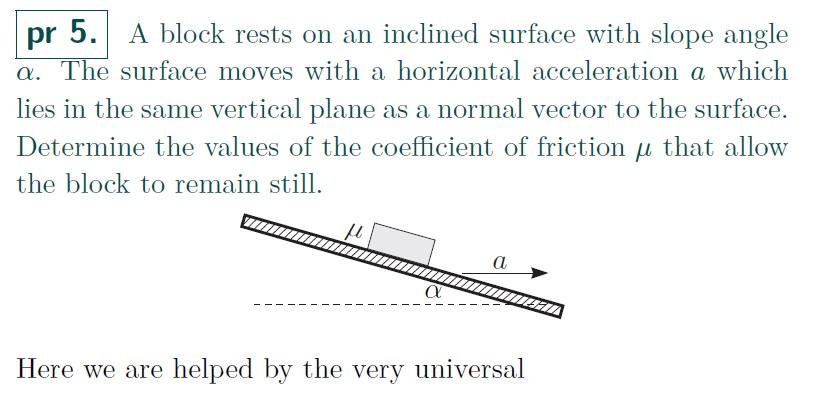
\includegraphics[scale=0.5]{pr 5.jpg}
    \end{wrapfigure}

    \textbf{Method 1} \quad
    To solve this problem, the common method would be to resolve forces
    Resolving forces along the slope gives us:
    $$mg\sin\alpha-f-ma\cos\alpha=0$$
    Resolving forces perpendicular to the slope gives us:
    $$N-mg\cos\alpha-ma\sin\alpha=0$$
    Since $N$ must be positive for the block to stay on the plane, we get the first inequality
    $$g\cos\alpha+a\sin\alpha > 0$$
    Our second inequality comes from the force balance along the slope, where $\mid f \mid\leq\mu N$
    So we get
    \begin{equation}
        \mu \geq \frac{\mid a\cos\alpha-g\sin\alpha \mid}{g\cos\alpha+a\sin\alpha}
    \end{equation}
    Both inequalities have to be satisfied for the block to remain on the slope.

    \tcblower
    \textbf{Method 2} \quad heheheh
\end{mybox}



\section{Tension}
\subsection{Rubber band around cylinder}
In fact, we have to
\begin{enumerate}
    \item Analyse an infinitesimal string element which subtends an angle of $d\theta$.
    \item It is not hard to see that the radial component is $T\sin\frac{d\theta}{2}$. By small angle approximation, which states that $sin\theta \approx \theta$ for small $\theta$, we get: $Td\theta$ (2 tensions acting on both ends)
    \item Integrate this tension from $0$ to $2 \pi $, the total tension would then be (look abit weird but I think it's correct) $2 \pi T$.
\end{enumerate}

\subsection{Hanging Chain}
\begin{mybox}{gray}{Example from \textbf{Morin 2.8}}
    \begin{enumerate}
        \item Realise that $T_x$ is constant throughout the chain, and $\frac{T_y}{T_x}=y'$. Hence, $T_y=T_x y' = C y'$
        \item And also realised that the mass of each infinitesimal chain segments can be expressed as such
              \begin{equation}
                  \rho \vec{g} dl= \rho \vec{g} \sqrt {dx^2+dy^2}=\rho \vec{g} \sqrt {1+y'^2}dx
              \end{equation}
        \item However, it is the \textbf{difference in tension} that balance out the wright. We can then write down the final relationships and solve the equation using substitution and separation of variables.
              \begin{equation}
                  d(Cy')= \rho \vec{g} \sqrt {1+y'^2}dx
              \end{equation}
              \begin{equation}
                  C y''= \rho \vec{g} \sqrt {1+y'^2}
              \end{equation}
    \end{enumerate}
\end{mybox}

\section{SHM}
\subsection{Translational perturbation}
\begin{enumerate}
    \item Find $\sum F$, and find all the equilibrium positions where $\sum F=0$ (these are the stable equilibriums)
    \item Use: $k=-\frac{dF}{dx}$. (negative sign depends on the direction of F. In this case, F is defined as positive in the direction that points away from equilibrium)
    \item Then do smth like $\frac{dF}{dx}\big|_{x=x_{\textsf{eqm}}}$, and substitute the values (Hookes constant $k$) into $\omega = \sqrt \frac{k}{m}$
\end{enumerate}

\subsection{Radial perturbation}
I am not sure about this, but this is what i see people do on PhOD to solve questions (physics olympiad discord)
\begin{enumerate}
    \item Let the small perturbation "displacement" be $\delta$.
    \item If the mass is revolving around some bigger object and the only force acting on it is in the radial direction, then we can use \textbf{conservation of angular momentum}
          \begin{equation}
              r^2\omega=(r+\delta)^2\omega'
          \end{equation}
          Through simple algebraic manipulation, we get
          \begin{equation}
              \omega'= \bigg(\frac{r}{r+\delta}\bigg)^2\omega
          \end{equation}
    \item In the rotating frame, we can write
          \begin{equation}
              m \frac{d^2 \delta}{dt^2}= m (r+\delta)\omega'^2-F_{\textsf{central}}
          \end{equation}
    \item Try to fit that to the classic SHM equation (maybe can simplify RHS and expand to first order in $\delta$): $\ddot{x}+\omega^2 x = 0$, and use $\omega = \sqrt \frac{k}{m}$
\end{enumerate}

\section{Non-inertial reference frames}
I think fictitious forces are just there to make sure that everything works on in non-inertial reference frames as well.
\subsection{Translational}
Let the lab frame be $S$, and the non inertial frame moving at $\vec{a_0}$ be $S'$. If the object's acceleration is $\vec{a}$ in the lab frame, its acceleration in the non-inertial frame would be $\vec{a}-\vec{a_0}=\vec{a'}$. The fictitious force present is thus $-m \vec{a_0}$. (translational force)

\subsection{Rotational}
Consider a system of reference, which rotates around the origin $O$ with an angular velocity $\boldsymbol{\omega}$. Consider a point $P$, which is motionless in the ortating system, and let us denote $\vec{r}=\vec{OP}$.
In the lab system of reference, the point $P$ moves with velocity $\mathbf{v}=\frac{d\mathbf{r}}{dt}=\mathbf{r} \times \boldsymbol{\omega}$. Now, if the point $P$ moves in the rotating frame of refernece with velocity $\mathbf{u}=\frac{d\mathbf{r}}{d\tau}$ ($\tau$ is used to emasure the time in the rotating system), then this additional velocity needs to be added to what should have been for a motionless point:
$$\frac{d\mathbf{r}}{dt}=\frac{d\mathbf{r}}{d\tau}+\boldsymbol{\omega}\times \mathbf{r}$$
So, we can conclude that the time-derivatives of vectors in rotating and lab frames of refernce are related via equality
$$\frac{d}{dt}=\frac{d\mathbf{r}}{d\tau}+\boldsymbol{\omega}\times . $$
This is written in the form of an operator, which means that we can write any vector (e.g. $\mathbf{r}$,$\mathbf{v}$) rightwards of all the three terms. In particular, we can apply this formula to the right and left hand sides of the equality $\mathbf{v}=\mathbf{u}+\boldsymbol{\omega} \times \mathbf{r}$

$$\frac{d\mathbf{v}}{dt}=\bigg(\frac{d}{d\tau}+\boldsymbol{\omega}\times\bigg)\bigg(\mathbf{u}+\boldsymbol{\omega}\times\mathbf{r}\bigg)
    \\
    = \frac{d\mathbf{u}}{d\tau}+\boldsymbol{\omega}\times\mathbf{u}+\frac{d(\boldsymbol{\omega}\times \mathbf{r})}{d\tau}+\boldsymbol{\omega}\times(\boldsymbol{\omega}\times \mathbf{r})$$
We obtain
$$\frac{d\mathbf{v}}{dt}=\frac{d\mathbf{u}}{d\tau}+2\boldsymbol{\omega}\times\mathbf{u}-\boldsymbol{\omega}^2\mathbf{r}$$

Recall that $\frac{d\mathbf{v}}{dt}$ is the acceleration of the point $P$ as seen in the lab frame of refernce, and $\frac{d\mathbf{u}}{d\tau}$ is the same as seen in the rotating frame of reference. now, if $P$ is a point mass $m$, and thee is an external force $\mathbf{F}$ acting on $P$, then $\mathbf{F}=m\frac{d\mathbf{v}}{dt}$ and hence,
$$m\frac{d\mathbf{u}}{d\tau}=\mathbf{F}-2\boldsymbol{\omega}\times\mathbf{u}m+\boldsymbol{\omega}^2\mathbf{r}m$$
\section{SJPO2021 Special Round Qn}
\begin{mybox}{gray}{Da question}

    \begin{wrapfigure}{l}{0.4\textwidth}
        \begin{tikzpicture}[x=0.75pt,y=0.75pt,yscale=-0.9,xscale=0.9]
            %uncomment if require: \path (0,300); %set diagram left start at 0, and has height of 300

            %Shape: Circle [id:dp19822565348906274] 
            \draw  [fill={rgb, 255:red, 215; green, 215; blue, 215 }  ,fill opacity=1 ] (149,40.4) .. controls (149,34.1) and (154.1,29) .. (160.4,29) .. controls (166.7,29) and (171.8,34.1) .. (171.8,40.4) .. controls (171.8,46.7) and (166.7,51.8) .. (160.4,51.8) .. controls (154.1,51.8) and (149,46.7) .. (149,40.4) -- cycle ;
            %Shape: Circle [id:dp3426728199976101] 
            \draw  [fill={rgb, 255:red, 215; green, 215; blue, 215 }  ,fill opacity=1 ] (149,136.4) .. controls (149,130.1) and (154.1,125) .. (160.4,125) .. controls (166.7,125) and (171.8,130.1) .. (171.8,136.4) .. controls (171.8,142.7) and (166.7,147.8) .. (160.4,147.8) .. controls (154.1,147.8) and (149,142.7) .. (149,136.4) -- cycle ;
            %Straight Lines [id:da8938425234356642] 
            \draw    (160.4,51.8) -- (160.4,125) ;
            %Straight Lines [id:da6191489683695304] 
            \draw [color={rgb, 255:red, 74; green, 93; blue, 226 }  ,draw opacity=1 ][line width=1.5]    (171.8,40.4) -- (205.83,39.91) -- (209.8,39.86) ;
            \draw [shift={(213.8,39.8)}, rotate = 539.1800000000001] [fill={rgb, 255:red, 74; green, 93; blue, 226 }  ,fill opacity=1 ][line width=0.08]  [draw opacity=0] (11.61,-5.58) -- (0,0) -- (11.61,5.58) -- cycle    ;
            %Shape: Axis 2D [id:dp15146894469957406] 
            \draw  (265,129.12) -- (351.8,129.12)(273.68,51) -- (273.68,137.8) (344.8,124.12) -- (351.8,129.12) -- (344.8,134.12) (268.68,58) -- (273.68,51) -- (278.68,58)  ;
            %Straight Lines [id:da5814568840159711] 
            \draw [color={rgb, 255:red, 208; green, 2; blue, 27 }  ,draw opacity=1 ][line width=1.5]    (288.8,51.4) -- (322.83,50.91) -- (326.8,50.86) ;
            \draw [shift={(330.8,50.8)}, rotate = 539.1800000000001] [fill={rgb, 255:red, 208; green, 2; blue, 27 }  ,fill opacity=1 ][line width=0.08]  [draw opacity=0] (11.61,-5.58) -- (0,0) -- (11.61,5.58) -- cycle    ;
            %Shape: Circle [id:dp4673346981336375] 
            \draw  [fill={rgb, 255:red, 215; green, 215; blue, 215 }  ,fill opacity=1 ] (325.26,74.86) .. controls (327.9,72.65) and (331.84,73.01) .. (334.04,75.65) .. controls (336.25,78.29) and (335.9,82.22) .. (333.26,84.43) .. controls (330.61,86.64) and (326.68,86.29) .. (324.47,83.64) .. controls (322.27,81) and (322.62,77.07) .. (325.26,74.86) -- cycle ;
            %Shape: Circle [id:dp48839595309985206] 
            \draw  [fill={rgb, 255:red, 215; green, 215; blue, 215 }  ,fill opacity=1 ] (284.96,108.53) .. controls (287.61,106.32) and (291.54,106.68) .. (293.75,109.32) .. controls (295.96,111.96) and (295.6,115.89) .. (292.96,118.1) .. controls (290.32,120.31) and (286.38,119.96) .. (284.18,117.32) .. controls (281.97,114.67) and (282.32,110.74) .. (284.96,108.53) -- cycle ;
            %Straight Lines [id:da5712778086817507] 
            \draw    (324.47,83.64) -- (293.75,109.32) ;
            %Flowchart: Summing Junction [id:dp33175257463483754] 
            \draw   (154,74) .. controls (154,70.47) and (156.87,67.6) .. (160.4,67.6) .. controls (163.93,67.6) and (166.8,70.47) .. (166.8,74) .. controls (166.8,77.53) and (163.93,80.4) .. (160.4,80.4) .. controls (156.87,80.4) and (154,77.53) .. (154,74) -- cycle ; \draw   (155.87,69.47) -- (164.93,78.53) ; \draw   (164.93,69.47) -- (155.87,78.53) ;
            %Flowchart: Summing Junction [id:dp6201575245730861] 
            \draw   (311.11,91.43) .. controls (311.11,89.03) and (313.06,87.08) .. (315.46,87.08) .. controls (317.85,87.08) and (319.8,89.03) .. (319.8,91.43) .. controls (319.8,93.83) and (317.85,95.77) .. (315.46,95.77) .. controls (313.06,95.77) and (311.11,93.83) .. (311.11,91.43) -- cycle ; \draw   (312.38,88.35) -- (318.53,94.5) ; \draw   (318.53,88.35) -- (312.38,94.5) ;
            %Straight Lines [id:da03269001228001933] 
            \draw    (126.8,40.6) -- (149,40.4) ;
            %Straight Lines [id:da1122374457863542] 
            \draw    (138.8,73.6) -- (160.4,74) ;
            %Straight Lines [id:da009815337614956343] 
            \draw    (126.8,136.6) -- (149,136.4) ;
            %Straight Lines [id:da44886965522336975] 
            \draw    (143.8,43.8) -- (143.8,70.8) ;
            \draw [shift={(143.8,73.8)}, rotate = 270] [fill={rgb, 255:red, 0; green, 0; blue, 0 }  ][line width=0.08]  [draw opacity=0] (5.36,-2.57) -- (0,0) -- (5.36,2.57) -- cycle    ;
            \draw [shift={(143.8,40.8)}, rotate = 90] [fill={rgb, 255:red, 0; green, 0; blue, 0 }  ][line width=0.08]  [draw opacity=0] (5.36,-2.57) -- (0,0) -- (5.36,2.57) -- cycle    ;
            %Straight Lines [id:da577760339017418] 
            \draw    (132.8,43.8) -- (132.8,132.8) ;
            \draw [shift={(132.8,135.8)}, rotate = 270] [fill={rgb, 255:red, 0; green, 0; blue, 0 }  ][line width=0.08]  [draw opacity=0] (5.36,-2.57) -- (0,0) -- (5.36,2.57) -- cycle    ;
            \draw [shift={(132.8,40.8)}, rotate = 90] [fill={rgb, 255:red, 0; green, 0; blue, 0 }  ][line width=0.08]  [draw opacity=0] (5.36,-2.57) -- (0,0) -- (5.36,2.57) -- cycle    ;
            %Curve Lines [id:da5841429723653924] 
            \draw    (324.8,62.8) .. controls (349.89,63.77) and (357.29,73.11) .. (352.38,97.13) ;
            \draw [shift={(351.8,99.8)}, rotate = 282.99] [fill={rgb, 255:red, 0; green, 0; blue, 0 }  ][line width=0.08]  [draw opacity=0] (7.14,-3.43) -- (0,0) -- (7.14,3.43) -- cycle    ;

            % Text Node
            \draw (162.4,135.4) node  [font=\scriptsize]  {$m_{1\ }$};
            % Text Node
            \draw (125.62,91.4) node    {$\mathrm{\ell }$};
            % Text Node
            \draw (182.4,43.3) node [anchor=north west][inner sep=0.75pt]  [color={rgb, 255:red, 74; green, 144; blue, 226 }  ,opacity=1 ]  {$u$};
            % Text Node
            \draw (161.4,39.4) node  [font=\scriptsize]  {$m_{2\ }$};
            % Text Node
            \draw (304.37,34.76) node  [color={rgb, 255:red, 74; green, 144; blue, 226 }  ,opacity=1 ]  {$\textcolor[rgb]{0.82,0.01,0.11}{v_{0}}$};
            % Text Node
            \draw (306.08,114.81) node  [font=\scriptsize,rotate=-359.24]  {$m_{1\ }$};
            % Text Node
            \draw (340.03,89.72) node  [font=\scriptsize,rotate=-1.09]  {$m_{2\ }$};
            % Text Node
            \draw (151.62,58.4) node    {$a$};
            % Text Node
            \draw (168,69) node [anchor=north west][inner sep=0.75pt]   [align=left] {{\fontfamily{cmss}\selectfont {\footnotesize COM}}};
            % Text Node
            \draw (363.37,69.76) node  [color={rgb, 255:red, 74; green, 144; blue, 226 }  ,opacity=1 ]  {$\textcolor[rgb]{0,0,0}{\mathbf{\omega }}$};
        \end{tikzpicture}
    \end{wrapfigure}

    Basically the question asks you to find the equation for the trajectory of the thing shown in the diagram when $m_2$ starts with an initial velocity $u$ perpendicular to the rod. (masses on frictionless ground). I think using the centre of mass frame would help in solving this problem.
    \hfill
\end{mybox}
Position of centre of mass with respect to $m_2$,
\begin{equation}
    a=\frac{m_1 \ell}{m_1+m_2}
\end{equation}
Velocity of centre of mass of the system can be calculated through conservation of momentum:
\begin{equation}
    v_{\textsf{COM}}=\frac{m_2u}{m_1+m_2}
\end{equation}
The moment of inertia of the system with respect to its centre of mass is
\begin{equation}
    I=m_2 \bigg(\frac{m_1 \ell}{m_1+m_2}\bigg)^2+m_1\bigg(\frac{m_2 \ell}{m_1+m_2}\bigg)^2=\frac{m_1 m_2 \ell^2}{m_1+m_2}
\end{equation}
Angular velocity could be either determined using \textbf{angular momentum}:
\begin{equation}
    \omega=\frac{L}{I}
\end{equation}
\begin{equation}
    \therefore\omega=\frac{u}{\ell}
\end{equation}
Or determined by \textbf{finding velocity of $m_2$ in the COM frame} and then \textbf{divide by the radius of rotation to find angular velocity} as $v=r\omega$.
\begin{equation}
    v'=u-\frac{m_2 u}{m_1+m_2}=\frac{m_1 u}{m_1+m_2}
\end{equation}
Dividing this by the radius of rotation (distance from $m_2$ to COM), we obtain the same expression for $\omega$
\begin{equation}
    \omega= \frac{v'}{a}=\frac{u}{\ell}
\end{equation}

Formulating the equation for trajectory:
\begin{equation}
    x(t)=a \sin (-\omega t)+v_{\textsf{COM}}t
\end{equation}
\begin{equation}
    y(t)=a \cos(\omega t)
\end{equation}
\begin{figure}[H]
    \centering
    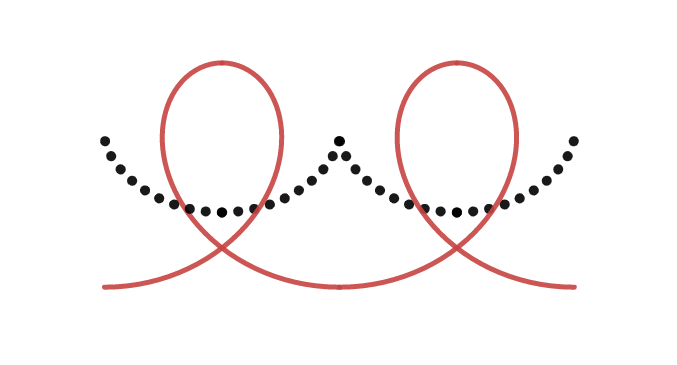
\includegraphics[width=10cm]{graph latex.jpeg}
    \caption{Trajectory plotted with Desmos}
    \label{fig:2}
\end{figure}

\section{Gravitation}
\section{Scaling and Parallel Axis theorem}
\subsection{MOI of a sierpinski triangle}

\def\trianglewidth{2cm}%
\pgfdeclarelindenmayersystem{Sierpinski triangle}{
    \symbol{X}{\pgflsystemdrawforward}
    \symbol{Y}{\pgflsystemdrawforward}
    \rule{X -> X-Y+X+Y-X}
    \rule{Y -> YY}
}
\foreach \level in {0,...,6}{
\tikzset{
    l-system={step=\trianglewidth/(2^\level), order=\level, angle=-120}
}
\begin{tikzpicture}
        \fill [black] (0,0) -- ++(0:\trianglewidth) -- ++(120:\trianglewidth) -- cycle;
        \draw [draw=none] (0,0) l-system
        [l-system={Sierpinski triangle, axiom=X},fill=white];
\end{tikzpicture}
}

\subsubsection{Building up}
We will build the triangle from the smallest triangle possible, and slowly work backwards. Let the smallest triangle be the basic repeating unit with mass $m$ and side length $\ell$. 

It is obvious that $m_{n+1}=3m_n$ and $\ell_{n+1}=2\ell_n$ with $I_{n+1}=3(I_n+m a^2)=3I_n+m\ell_n^2$ where a is the distance from the COM of the small triangle to that of the big triangle and is $\ell_n/\sqrt{3}$

The moment inertia can then be found through iterations,
\begin{align}
    I_1 
    &= 3Cm_0\ell_0^2+m_0^2\ell_0^2 = (3C+1)m_0\ell_0^2\nonumber\\
    I_2 &= 3I_1+m_1\ell_1^2=(3^2C+3+12)m_0\ell_0^2\nonumber\\
    I_3 &= 3I_2+m_2\ell_2^2=(3^2C+3^2+3\time 12+12^2)m_0\ell_0^2\nonumber\\
    I_n &= 3I_{n-1}+m_{n-1}\ell_{n-1}^2=(12^{n-1}+12^{n-2}3+...+3^{n-1}+3^n C)m_0\ell_0^2
\end{align}
where $Cm_0\ell_0^2$ is the moment of inertia of the basic building block

Taking the limits as $n\to\infty$
\begin{equation}
    \lim_{n\to\infty}I_n=12^{n-1}m_0\ell_0^2\bigg(1+\frac{1}{4}+\frac{1}{4^2}+...+\frac{1}{4^{n-1}}+\frac{1}{4^n}C\bigg)
\end{equation}
We note that the last term with $C$ plays no role in this infinite geometric series. After defining $\lim_{n\to\infty} 3^n m_0=M $ and $\lim_{n\to\infty} 2^n \ell_0=\ell$, and simplifying the above expression, we get

\begin{equation}
    \lim_{n\to\infty}I_n=\frac{1}{9}M\ell^2
\end{equation}

\subsubsection{Repeating pattern}
For a 2D-planar object (this is also from Ryan's lesson), the moment of inertia is calculated using 
\begin{equation}
    I=\int r^2 dm =\int r^2 \sigma dx dy
\end{equation}

where $\sigma$ is the surface mass density. We see that if we were to scale the side length of the planar object by 2 (or just scale it up by 2 times), the moment of inertia will be scaled up by $2^2 \times 2 \times 2=16$, due to the $r^2 dx dy$ in the above integral. 

However, the tricky part is that for a sierpinski triangle, it is a bit different. Because the $\sigma$ is always changing. Instead, we can rewrite $I$ as 
\begin{equation}
    I=\int r^2 dm
\end{equation}
If we were to scale up the triangle by 2 (go up by 1 layer), $r^2 dm$ will be equivalent to scaling $I$ up by $2^2 \times 3= 12$ times. 

so let the moment of inertia of one infinite siepinski triangle be $I$ with side length $\ell$. We know that we can form a bigger siepinski triangle (side length: $2\ell$) with 3 smaller ones. With this method, we arrive at the same answer
\begin{align}
    (2^2\times 3) I &= 3I+ m \ell^2\\
    I&=\frac{1}{9}m \ell^2
\end{align}

\begin{tikzpicture}
    \penguin
\end{tikzpicture}